\ifx\du\undefined
  \newlength{\du}
\fi
\setlength{\du}{15\unitlength}
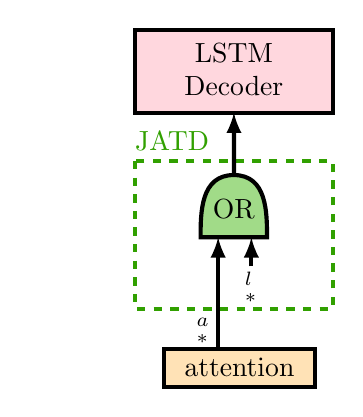
\begin{tikzpicture}[even odd rule]
\pgftransformxscale{1.000000}
\pgftransformyscale{-1.000000}
\definecolor{dialinecolor}{rgb}{0.000000, 0.000000, 0.000000}
\pgfsetstrokecolor{dialinecolor}
\pgfsetstrokeopacity{1.000000}
\definecolor{diafillcolor}{rgb}{1.000000, 1.000000, 1.000000}
\pgfsetfillcolor{diafillcolor}
\pgfsetfillopacity{1.000000}
\pgfsetlinewidth{0.100000\du}
\pgfsetdash{{0.200000\du}{0.200000\du}}{0\du}
\pgfsetmiterjoin
{\pgfsetcornersarced{\pgfpoint{0.000000\du}{0.000000\du}}\definecolor{diafillcolor}{rgb}{0.000000, 0.000000, 0.000000}
\pgfsetfillcolor{diafillcolor}
\pgfsetfillopacity{0.000000}
\fill (4.200000\du,3.763660\du)--(4.200000\du,7.317587\du)--(8.958597\du,7.317587\du)--(8.958597\du,3.763660\du)--cycle;
}{\pgfsetcornersarced{\pgfpoint{0.000000\du}{0.000000\du}}\definecolor{dialinecolor}{rgb}{0.192157, 0.627451, 0.000000}
\pgfsetstrokecolor{dialinecolor}
\pgfsetstrokeopacity{1.000000}
\draw (4.200000\du,3.763660\du)--(4.200000\du,7.317587\du)--(8.958597\du,7.317587\du)--(8.958597\du,3.763660\du)--cycle;
}% setfont left to latex
\definecolor{dialinecolor}{rgb}{0.192157, 0.627451, 0.000000}
\pgfsetstrokecolor{dialinecolor}
\pgfsetstrokeopacity{1.000000}
\definecolor{diafillcolor}{rgb}{0.192157, 0.627451, 0.000000}
\pgfsetfillcolor{diafillcolor}
\pgfsetfillopacity{1.000000}
\node[anchor=base east,inner sep=0pt, outer sep=0pt,color=dialinecolor] at (8.608597\du,5.734686\du){};
\pgfsetlinewidth{0.100000\du}
\pgfsetdash{}{0pt}
\pgfsetmiterjoin
\pgfsetbuttcap
\definecolor{diafillcolor}{rgb}{0.631373, 0.858824, 0.533333}
\pgfsetfillcolor{diafillcolor}
\pgfsetfillopacity{1.000000}
\definecolor{dialinecolor}{rgb}{0.000000, 0.000000, 0.000000}
\pgfsetstrokecolor{dialinecolor}
\pgfsetstrokeopacity{1.000000}
\pgfpathmoveto{\pgfpoint{7.377110\du}{5.600000\du}}
\pgfpathcurveto{\pgfpoint{6.843780\du}{5.600000\du}}{\pgfpoint{6.310440\du}{5.600000\du}}{\pgfpoint{5.777110\du}{5.600000\du}}
\pgfpathcurveto{\pgfpoint{5.777110\du}{5.000000\du}}{\pgfpoint{5.777110\du}{4.100000\du}}{\pgfpoint{6.577110\du}{4.100000\du}}
\pgfpathcurveto{\pgfpoint{7.377110\du}{4.100000\du}}{\pgfpoint{7.377110\du}{5.000000\du}}{\pgfpoint{7.377110\du}{5.600000\du}}
\pgfpathclose
\pgfusepath{fill,stroke}
\pgfsetlinewidth{0.100000\du}
\pgfsetdash{}{0pt}
\pgfsetmiterjoin
{\pgfsetcornersarced{\pgfpoint{0.000000\du}{0.000000\du}}\definecolor{diafillcolor}{rgb}{1.000000, 0.843137, 0.870588}
\pgfsetfillcolor{diafillcolor}
\pgfsetfillopacity{1.000000}
\fill (4.201490\du,0.600000\du)--(4.201490\du,2.600000\du)--(8.957108\du,2.600000\du)--(8.957108\du,0.600000\du)--cycle;
}{\pgfsetcornersarced{\pgfpoint{0.000000\du}{0.000000\du}}\definecolor{dialinecolor}{rgb}{0.000000, 0.000000, 0.000000}
\pgfsetstrokecolor{dialinecolor}
\pgfsetstrokeopacity{1.000000}
\draw (4.201490\du,0.600000\du)--(4.201490\du,2.600000\du)--(8.957108\du,2.600000\du)--(8.957108\du,0.600000\du)--cycle;
}% setfont left to latex
\definecolor{dialinecolor}{rgb}{0.000000, 0.000000, 0.000000}
\pgfsetstrokecolor{dialinecolor}
\pgfsetstrokeopacity{1.000000}
\definecolor{diafillcolor}{rgb}{0.000000, 0.000000, 0.000000}
\pgfsetfillcolor{diafillcolor}
\pgfsetfillopacity{1.000000}
\node[anchor=base,inner sep=0pt, outer sep=0pt,color=dialinecolor] at (6.579299\du,1.394062\du){LSTM};
% setfont left to latex
\definecolor{dialinecolor}{rgb}{0.000000, 0.000000, 0.000000}
\pgfsetstrokecolor{dialinecolor}
\pgfsetstrokeopacity{1.000000}
\definecolor{diafillcolor}{rgb}{0.000000, 0.000000, 0.000000}
\pgfsetfillcolor{diafillcolor}
\pgfsetfillopacity{1.000000}
\node[anchor=base,inner sep=0pt, outer sep=0pt,color=dialinecolor] at (6.579299\du,2.194063\du){Decoder};
\pgfsetlinewidth{0.100000\du}
\pgfsetdash{}{0pt}
\pgfsetbuttcap
{
\definecolor{diafillcolor}{rgb}{0.000000, 0.000000, 0.000000}
\pgfsetfillcolor{diafillcolor}
\pgfsetfillopacity{1.000000}

\pgfsetarrowsend{latex}
\definecolor{dialinecolor}{rgb}{0.000000, 0.000000, 0.000000}
\pgfsetstrokecolor{dialinecolor}
\pgfsetstrokeopacity{1.000000}
\draw (6.583080\du,4.096640\du)--(6.579300\du,2.600000\du);
}
% setfont left to latex
\definecolor{dialinecolor}{rgb}{0.192157, 0.627451, 0.000000}
\pgfsetstrokecolor{dialinecolor}
\pgfsetstrokeopacity{1.000000}
\definecolor{diafillcolor}{rgb}{0.192157, 0.627451, 0.000000}
\pgfsetfillcolor{diafillcolor}
\pgfsetfillopacity{1.000000}
\node[anchor=base west,inner sep=0pt,outer sep=0pt,color=dialinecolor] at (4.200000\du,3.500000\du){JATD};
\pgfsetlinewidth{0.100000\du}
\pgfsetdash{}{0pt}
\pgfsetbuttcap
{
\definecolor{diafillcolor}{rgb}{0.000000, 0.000000, 0.000000}
\pgfsetfillcolor{diafillcolor}
\pgfsetfillopacity{1.000000}

\pgfsetarrowsend{latex}
\definecolor{dialinecolor}{rgb}{0.000000, 0.000000, 0.000000}
\pgfsetstrokecolor{dialinecolor}
\pgfsetstrokeopacity{1.000000}
\draw (6.200000\du,8.300000\du)--(6.200000\du,5.600000\du);
}
\pgfsetlinewidth{0.100000\du}
\pgfsetdash{}{0pt}
\pgfsetbuttcap
{
\definecolor{diafillcolor}{rgb}{0.000000, 0.000000, 0.000000}
\pgfsetfillcolor{diafillcolor}
\pgfsetfillopacity{1.000000}

\pgfsetarrowsend{latex}
\definecolor{dialinecolor}{rgb}{0.000000, 0.000000, 0.000000}
\pgfsetstrokecolor{dialinecolor}
\pgfsetstrokeopacity{1.000000}
\draw (7.000000\du,6.300000\du)--(7.000000\du,5.600000\du);
}
\pgfsetlinewidth{0.000000\du}
\pgfsetdash{}{0pt}
\pgfsetmiterjoin
{\pgfsetcornersarced{\pgfpoint{0.000000\du}{0.000000\du}}\definecolor{diafillcolor}{rgb}{0.000000, 0.000000, 0.000000}
\pgfsetfillcolor{diafillcolor}
\pgfsetfillopacity{0.000000}
\fill (1.611430\du,7.088820\du)--(1.611430\du,8.488820\du)--(6.202015\du,8.488820\du)--(6.202015\du,7.088820\du)--cycle;
}{\pgfsetcornersarced{\pgfpoint{0.000000\du}{0.000000\du}}\definecolor{dialinecolor}{rgb}{0.000000, 0.000000, 0.000000}
\pgfsetstrokecolor{dialinecolor}
\pgfsetstrokeopacity{0.000000}
\draw (1.611430\du,7.088820\du)--(1.611430\du,8.488820\du)--(6.202015\du,8.488820\du)--(6.202015\du,7.088820\du)--cycle;
}% setfont left to latex
\definecolor{dialinecolor}{rgb}{0.000000, 0.000000, 0.000000}
\pgfsetstrokecolor{dialinecolor}
\pgfsetstrokeopacity{1.000000}
\definecolor{diafillcolor}{rgb}{0.000000, 0.000000, 0.000000}
\pgfsetfillcolor{diafillcolor}
\pgfsetfillopacity{1.000000}
\node[anchor=base east,inner sep=0pt, outer sep=0pt,color=dialinecolor] at (6.002015\du,7.982882\du){$\vc_*^a$};
\pgfsetlinewidth{0.000000\du}
\pgfsetdash{}{0pt}
\pgfsetmiterjoin
{\pgfsetcornersarced{\pgfpoint{0.000000\du}{0.000000\du}}\definecolor{diafillcolor}{rgb}{0.000000, 0.000000, 0.000000}
\pgfsetfillcolor{diafillcolor}
\pgfsetfillopacity{0.000000}
\fill (5.400000\du,6.400000\du)--(5.400000\du,7.200000\du)--(8.592500\du,7.200000\du)--(8.592500\du,6.400000\du)--cycle;
}{\pgfsetcornersarced{\pgfpoint{0.000000\du}{0.000000\du}}\definecolor{dialinecolor}{rgb}{0.000000, 0.000000, 0.000000}
\pgfsetstrokecolor{dialinecolor}
\pgfsetstrokeopacity{0.000000}
\draw (5.400000\du,6.400000\du)--(5.400000\du,7.200000\du)--(8.592500\du,7.200000\du)--(8.592500\du,6.400000\du)--cycle;
}% setfont left to latex
\definecolor{dialinecolor}{rgb}{0.000000, 0.000000, 0.000000}
\pgfsetstrokecolor{dialinecolor}
\pgfsetstrokeopacity{1.000000}
\definecolor{diafillcolor}{rgb}{0.000000, 0.000000, 0.000000}
\pgfsetfillcolor{diafillcolor}
\pgfsetfillopacity{1.000000}
\node[anchor=base,inner sep=0pt, outer sep=0pt,color=dialinecolor] at (6.996250\du,6.994063\du){$\vc_*^l$};
\pgfsetlinewidth{0.100000\du}
\pgfsetdash{}{0pt}
\pgfsetmiterjoin
{\pgfsetcornersarced{\pgfpoint{0.000000\du}{0.000000\du}}\definecolor{diafillcolor}{rgb}{1.000000, 0.886275, 0.713726}
\pgfsetfillcolor{diafillcolor}
\pgfsetfillopacity{1.000000}
\fill (4.900000\du,8.300000\du)--(4.900000\du,9.200000\du)--(8.525688\du,9.200000\du)--(8.525688\du,8.300000\du)--cycle;
}{\pgfsetcornersarced{\pgfpoint{0.000000\du}{0.000000\du}}\definecolor{dialinecolor}{rgb}{0.000000, 0.000000, 0.000000}
\pgfsetstrokecolor{dialinecolor}
\pgfsetstrokeopacity{1.000000}
\draw (4.900000\du,8.300000\du)--(4.900000\du,9.200000\du)--(8.525688\du,9.200000\du)--(8.525688\du,8.300000\du)--cycle;
}% setfont left to latex
\definecolor{dialinecolor}{rgb}{0.000000, 0.000000, 0.000000}
\pgfsetstrokecolor{dialinecolor}
\pgfsetstrokeopacity{1.000000}
\definecolor{diafillcolor}{rgb}{0.000000, 0.000000, 0.000000}
\pgfsetfillcolor{diafillcolor}
\pgfsetfillopacity{1.000000}
\node[anchor=base,inner sep=0pt, outer sep=0pt,color=dialinecolor] at (6.712844\du,8.944063\du){attention};
\pgfsetlinewidth{0.100000\du}
\pgfsetdash{}{0pt}
\pgfsetmiterjoin
{\pgfsetcornersarced{\pgfpoint{0.000000\du}{0.000000\du}}\definecolor{diafillcolor}{rgb}{1.000000, 0.843137, 0.870588}
\pgfsetfillcolor{diafillcolor}
\pgfsetfillopacity{0.000000}
\fill (5.833830\du,4.173760\du)--(5.833830\du,5.726926\du)--(7.318673\du,5.726926\du)--(7.318673\du,4.173760\du)--cycle;
}{\pgfsetcornersarced{\pgfpoint{0.000000\du}{0.000000\du}}\definecolor{dialinecolor}{rgb}{0.000000, 0.000000, 0.000000}
\pgfsetstrokecolor{dialinecolor}
\pgfsetstrokeopacity{0.000000}
\draw (5.833830\du,4.173760\du)--(5.833830\du,5.726926\du)--(7.318673\du,5.726926\du)--(7.318673\du,4.173760\du)--cycle;
}% setfont left to latex
\definecolor{dialinecolor}{rgb}{0.000000, 0.000000, 0.000000}
\pgfsetstrokecolor{dialinecolor}
\pgfsetstrokeopacity{1.000000}
\definecolor{diafillcolor}{rgb}{0.000000, 0.000000, 0.000000}
\pgfsetfillcolor{diafillcolor}
\pgfsetfillopacity{1.000000}
\node[anchor=base,inner sep=0pt, outer sep=0pt,color=dialinecolor] at (6.576252\du,5.144406\du){OR};
\end{tikzpicture}
